\documentclass{article}

% Language setting
% Replace `english' with e.g. `spanish' to change the document language
\usepackage[english]{babel}

% Set page size and margins
% Replace `letterpaper' with`a4paper' for UK/EU standard size
\usepackage[letterpaper,top=2cm,bottom=2cm,left=3cm,right=3cm,marginparwidth=1.75cm]{geometry}

% Useful packages
\usepackage{amsmath}
\usepackage{graphicx}
\usepackage[colorlinks=true, allcolors=blue]{hyperref}
\usepackage{subcaption}

\title{Mushroom Edibility Classification Data Anlysis}
\author{Yanfeiyun (Kathy) Wu\\
\textit{\small Data Science Institute, Brown University}\\
\href{https://github.com/kathywu1201/Mushroom_Edibility_Classification_ML_Project}{\small https://github.com/kathywu1201/Mushroom\_Edibility\_Classification\_ML\_Project}}


\begin{document}
\maketitle

\section{Introduction}

\hspace{0.5cm} Mushroom poisoning has become a serious food safety issue in China. According to the investigation of China CDC, in 2022, there are 482 mushroom poisoning incidents involving 1,332 patients and 28 deaths, with a total case fatality rate of 2.1\% \cite{Li et al.}. In view of the extensive impact and harm of poisonous mushrooms on public health, it is necessary to promote prevention and most importantly improve the ability of professionals to identify and diagnose mushroom poisoning. In addition to the current existing mushroom species, it is possible that there might appear a new mushroom that was not recorded, how should we categorize this mushroom, edible or poisonous? As a result, in building up this Mushroom classification Machine Learning model, we can potentially reduce the risk of death and intoxication due to poisonous mushroom.

This Mushroom Edibility Classification Dataset \cite{Zohaib} was found in Kaggle, collected from Patrick Hardin’s Mushrooms \& Toadstools, and inspired by Jeff Schlimmer’s Mushroom Data Set . This dataset includes 61069 hypothetical mushrooms with caps based on 173 species where each mushroom is identified as definitely edible, definitely poisonous, or of unknown edibility which is classified as poisonous.

The Mushroom Edibility Classification Dataset is a classification which originally contains 61069 observations and 21 features including the target variable ‘class.’ In the ‘class’ variable, ‘e’ meaning edible is encoded as 0 and ‘p’ meaning poisonous is encoded as 1 in preprocessing. 

In the recent two Kaggle projects centered on the Mushroom Edibility Classification Dataset, different machine learning models were employed to determine the edibility of mushrooms. Lucas Agra utilized a Random Forest Model, achieving remarkable predictive power with a 100\% accuracy rate \cite{Agra}. In addition, Levi Payne opted for the XGBoost model in their analysis of the same dataset, demonstrating a high level of accuracy with a score of 99.96\% \cite{Payne}. These results highlight the effectiveness of both Random Forest and XGBoost models in accurately classifying mushroom edibility.

\section{Exploratory Data Analysis}
\hspace{0.5cm} In the initial phase of the project, I conducted a comprehensive exploratory data analysis (EDA) to gain valuable insights into the characteristics and patterns within the mushroom dataset. Starting with an analysis of the distribution of the target variable, Figure 1(a) reveals that the ratio of the target variable is approximately 6:4 for poisonous and edible instances, respectively. 

When inspecting the missing values in the dataset, we found that among the 20 features, 9 categorical features contain missing values, with 5 features having more than 60\% of missing values (see Figure 1(b)). However, we decided to keep all of them, as missing values in these features indicate that some mushrooms do not have certain features. Yet, this does not necessarily imply that an unseen mushroom lacks these features either.

\begin{figure}[ht]
  \begin{subfigure}{0.5\textwidth}
    \centering
        \centering
        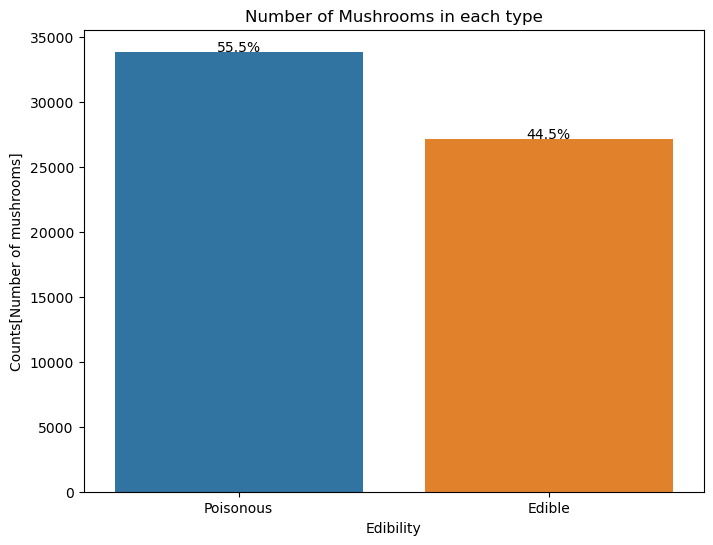
\includegraphics[width=\textwidth]{eda_target.png}
        \caption{\label{fig:target variable} Distribution of target variables.}
  \end{subfigure}%
  \hfill
  \begin{subfigure}{0.48\textwidth}

    \begin{tabular}{|l|l|} \hline
        \textbf{Feature} & \textbf{Percentage of Missing} \\
        (categorical features) & \\\hline
        cap-surface & 0.231214 \\\hline
        gill-attachment & 0.161850 \\\hline
        gill-spacing & 0.410405 \\\hline
        stem-root & 0.843931 \\\hline
        stem-surface & 0.624277 \\\hline
        veil-type & 0.947977 \\\hline
        veil-color & 0.878613 \\\hline
        ring-type & 0.040462 \\\hline
        spore-print-color & 0.895954 \\ \hline
    \end{tabular}
    \caption{\label{tab:widgets} Percentage of missing value in each feature.}
  \end{subfigure}
  \caption{Target variable distribution \& Percentage of missing value}
\end{figure}

\newpage
According to the Boxplot of Cap Diameter Based on Different Cap Shape (see Figure 2), the bell cap shape mushroom overall have a small cap-diameter while the spherical cap shape mushroom relatively have a large cap-diameter.

\begin{figure}[h]
\centering
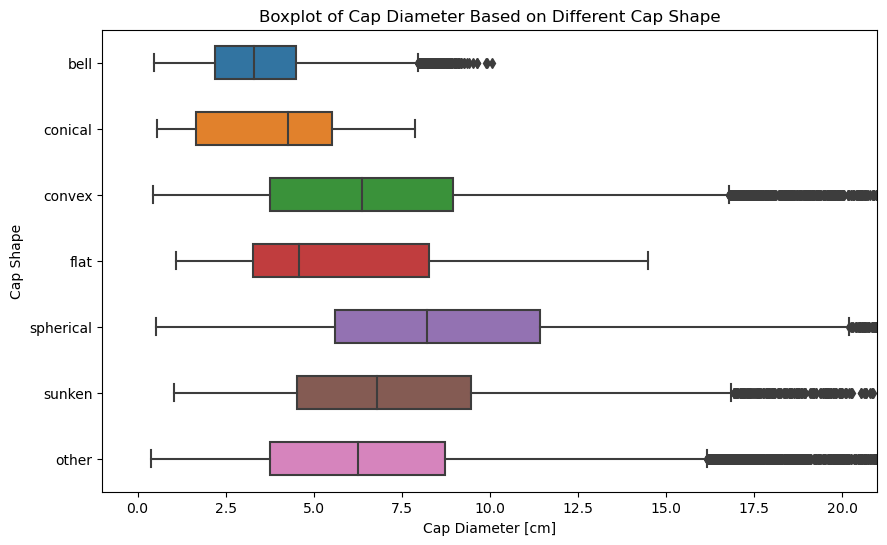
\includegraphics[width=0.8\textwidth]{eda1.png}
\caption{\label{fig:boxplot} Boxplot of cap shape vs. cap diameter.}
\end{figure}

In this stacked bar plot calculating the percentage of edible and poisonous mushroom based on the habitat of mushroom (see Figure 3), is appears to have 100\% of edible mushroom grown in urban and waste area, and 100\% of poisonous mushroom grown in paths area according to the dataset. 

\begin{figure}[h]
\centering
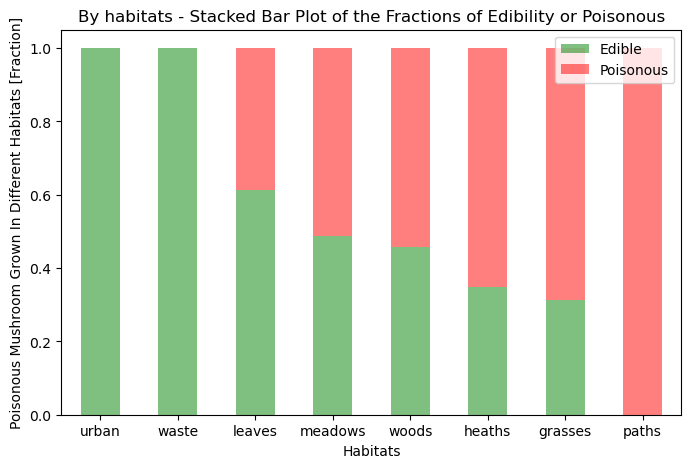
\includegraphics[width=0.8\textwidth]{eda2.png}
\caption{\label{fig:boxplot} Stacked Bar Plot of mushroom edibility based on habitat.}
\end{figure}

\newpage
This category specific histogram on stem width (see Figure 4) demonstrates that the edible and poisonous mushroom have two different peak regarding the stem width. A mushroom with wider stem width seems to be less pernicious than those with thinner stem width.

\begin{figure}[h]
\centering
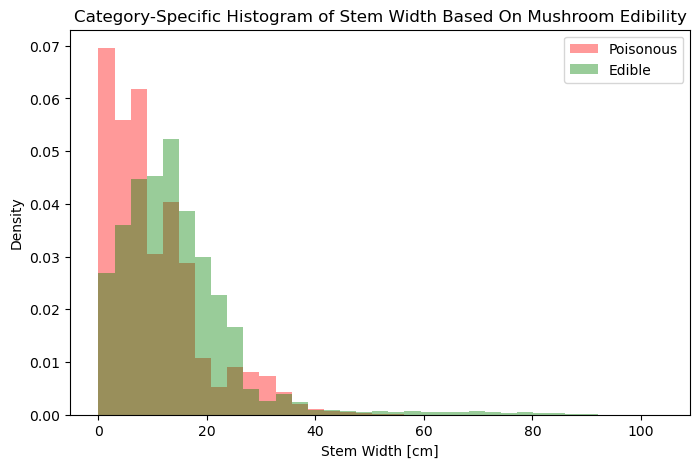
\includegraphics[width=0.77\textwidth]{eda3.png}
\caption{\label{fig:histogram} Category Specific Histogram on stem width.}
\end{figure}


\section{Methods}

\subsection{Data Splitting}

\hspace{0.5cm} The Mushroom Edibility Classification dataset exhibits relatively balanced target variable classes, with a ratio of approximately 4 to 6 for the edible and poisonous classes, respectively. The general train\_test\_split is applied first then using Kfold cross validation with 4 splits. After splitting, there will be 80\% of (train set + validation set) and 20\% of test set.

\subsection{Data Preprocessing}
\hspace{0.5cm} The dataset contains a total of 20 features for prediction, while 3 of them are continuous features and 17 of them are categorical features. For the continuous features, all of them follows a heavy-tailed distribution (see Figure 5) and are not bounded. Therefore, 2 preprocessors - one-hot encoder and standard scalars- are applied to the dataset. After preprocessing, the dataset contains 124 features and no feature has missing value.

\begin{figure}[h]
\centering
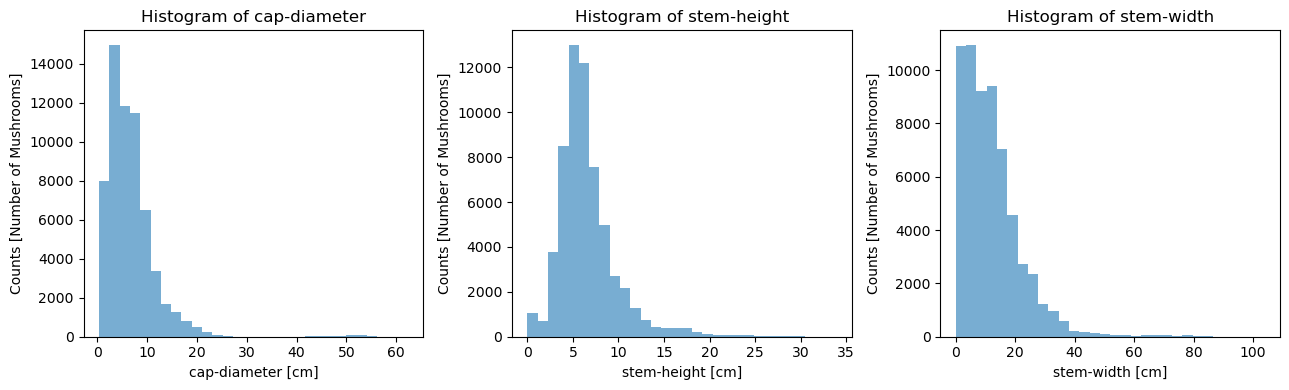
\includegraphics[width=1\textwidth]{hist1.png}
\caption{\label{fig:frog} Histograms showing heavy-tailed distribution of continuous features.}
\end{figure}

\subsection{Evaluation Metric}
\hspace{0.5cm} The Accuracy Score serves as the evaluation metric to examine the model's performance. Accuracy, a straightforward and intuitive measure, represents the proportion of correctly classified instances over the total number of instances. Given the balanced nature of this mushroom dataset, accuracy provides a clear and easily interpretable metric for overall model performance.  

\subsection{Machine Learning Models}
\hspace{0.5cm} In this classification problem, five machine learning models are utilized. The models and tuned parameters are in the following Table:

\begin{table}[h]
\centering
\begin{tabular}{|l|l|} \hline
\textbf{Machine Learning Model} & \textbf{Parameter(s)} \\\hline
Logistic Regression & C = 1/alpha: $[1/0.001, 1/0.01, 1/0.1, 1/1.0]$\\ \hline
Random Forest & max\_depth: [5, 10, 20, 30] \\
 & max\_features: [0.25, 0.5, 0.75, 1.0] \\
 & n\_estimators: [20, 50, 100] \\ \hline
K Nearest Neighbors (KNN) & n\_neighbors: [3,9,12,15,30,50,100] \\ \hline
XGBoost & max\_depth: [3, 5, 7, 10] \\
 & min\_child\_weight: [1, 3, 5] \\
 & learning\_rate: [0.1] \\
 & lambda: [0.01, 0.1, 1] \\
 & alpha: [0.01, 0.1, 1] \\ \hline
Support Vector Classification (SVC) &  gamma: [1e-2, 1e-1, 1e1, 1e3] \\
 & C: [1e-1, 1e0, 1e1, 1e2] \\ \hline
\end{tabular}
\caption{\label{tab:widgets} The parameters tuned for each model.}
\end{table}

\subsection{Machine Learning Pipeline}
\hspace{0.5cm} To achieve hyper-parameter tuning, GridSearchCV is used to find the best set of parameters for a model by evaluating the model's performance using cross-validation. For each model, 5 different random states are assigned to each splitting to generalize the resulitng test scores. First, general train-test-split is applied to split the dataset into test set and other set. Then, in the gridsearchCV, it will evaluate the accuracy score for each set of parameters and for each splits. Then it will find the best parameters with the highest accuracy score. After that, it will evaluate the test score using the best parameters (see Figure 6). 

In addition, in the XGBoost algorithm, similar pipeline is considered but early\_stopping is added to halt the training process when the performance of the model on a validation dataset stops improving, avoiding the risk of overfitting.

\begin{figure}[h]
\centering
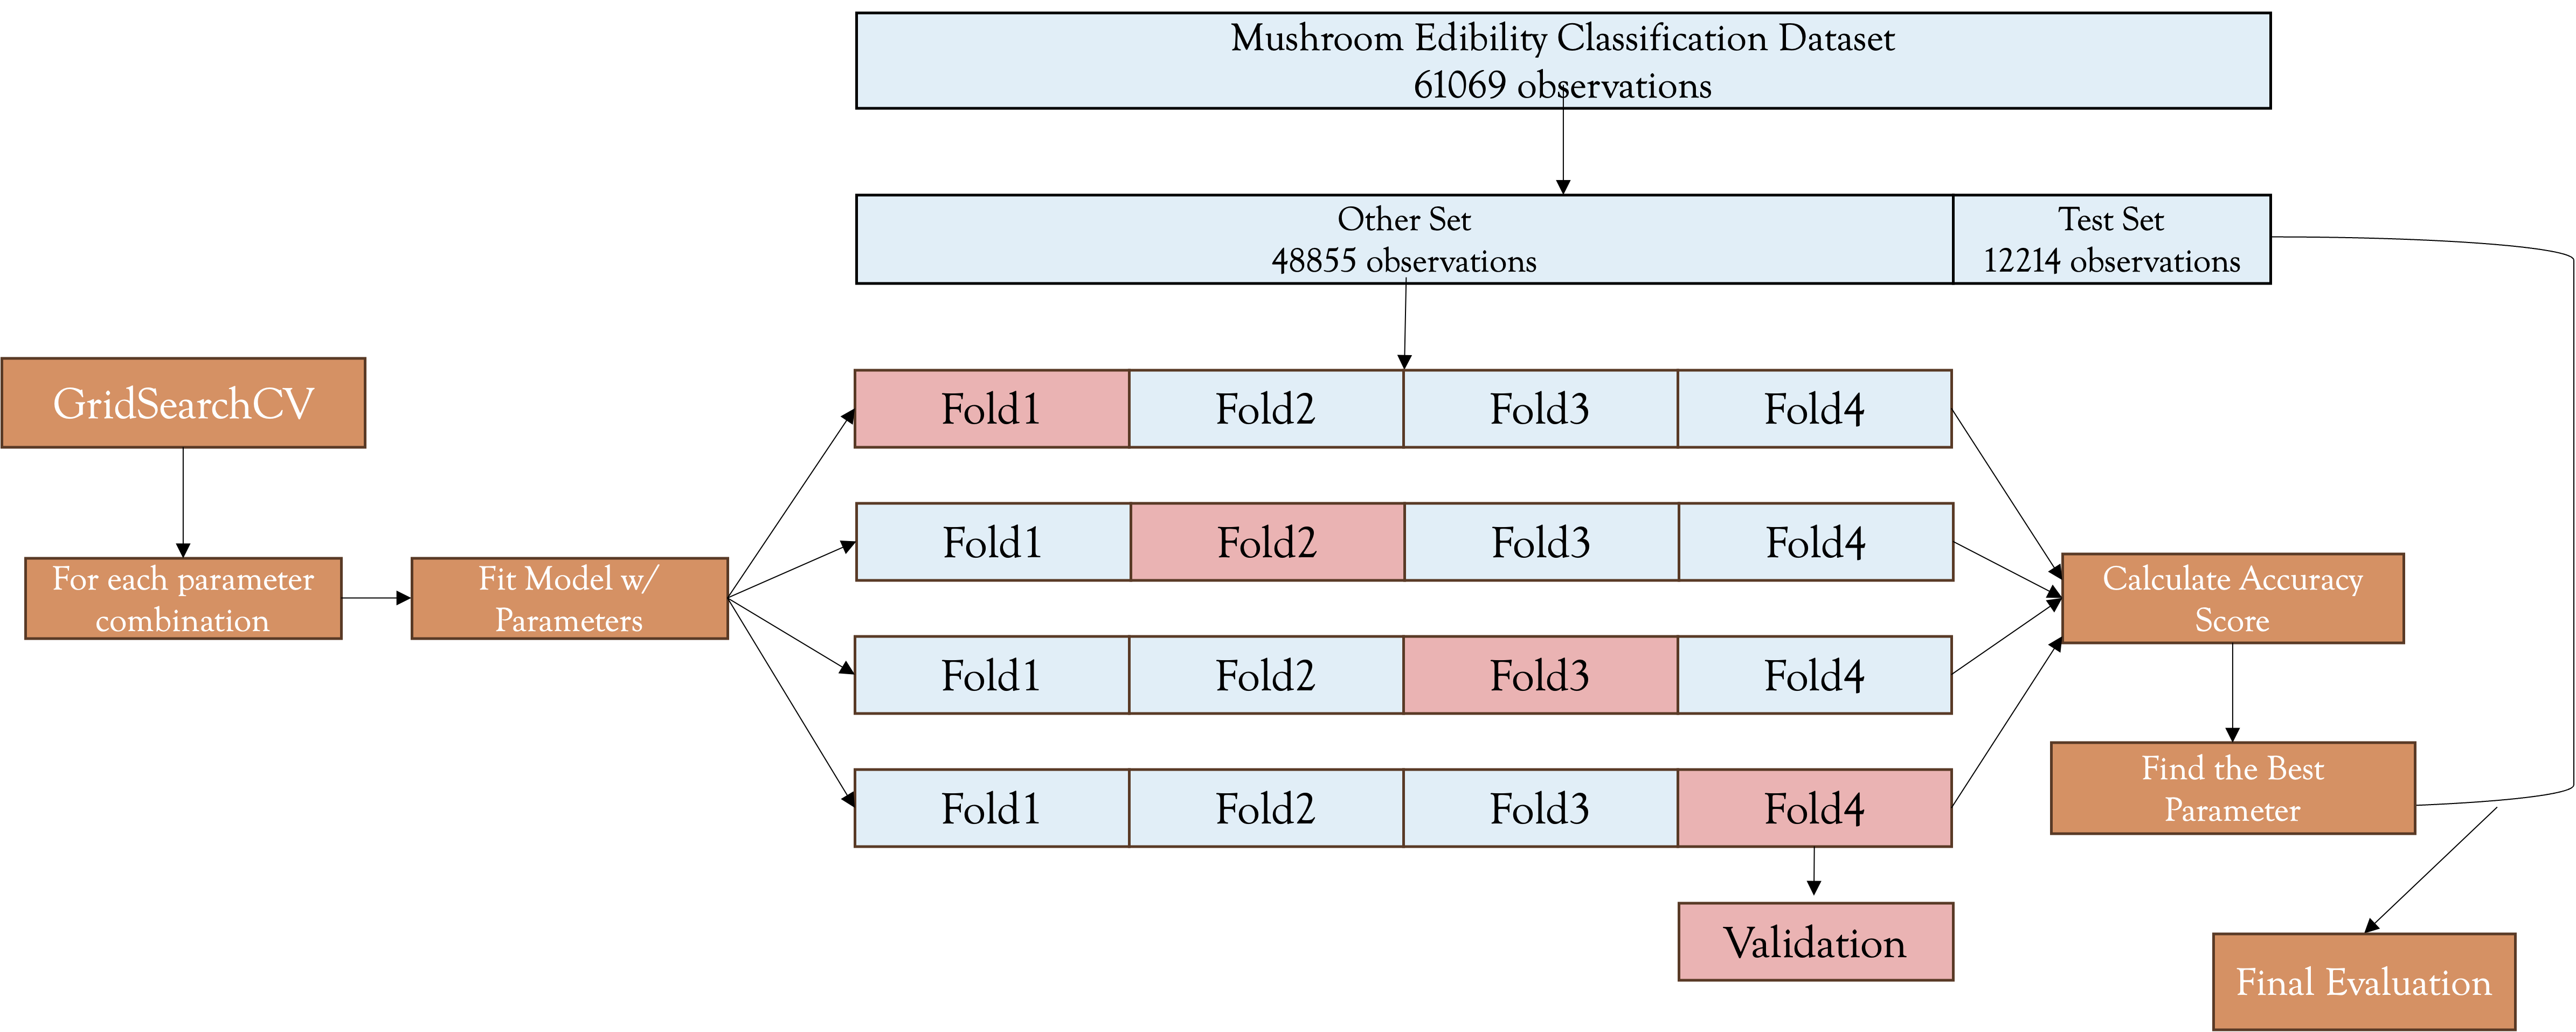
\includegraphics[width=1\textwidth]{ml_pipeline.png}
\caption{\label{fig:frog} Visualization of finding the best set of parameters using GridSearchCV.}
\end{figure}

\section{Results}

\subsection{Models' Performance}
\hspace{0.5cm} According to the mean test scores of the models evaluated on the test sets, \textbf{K Nearest Neighbors} appears to obtain the highest accuracy score (see Table 2). However, the test accuracy score of Logistic Regression is significantly different from that of other models, with a lowest accuracy score of 0.86 (see Figure 7(a)), while the other non-linear models achieve scores approximately equal to 0.99 (see Figure 7(b)). This strongly suggests that this dataset is non-linear and works better with tree-based models and non-parametric models.

\begin{figure}[h]
    \centering
    \begin{subfigure}{0.46\textwidth}
        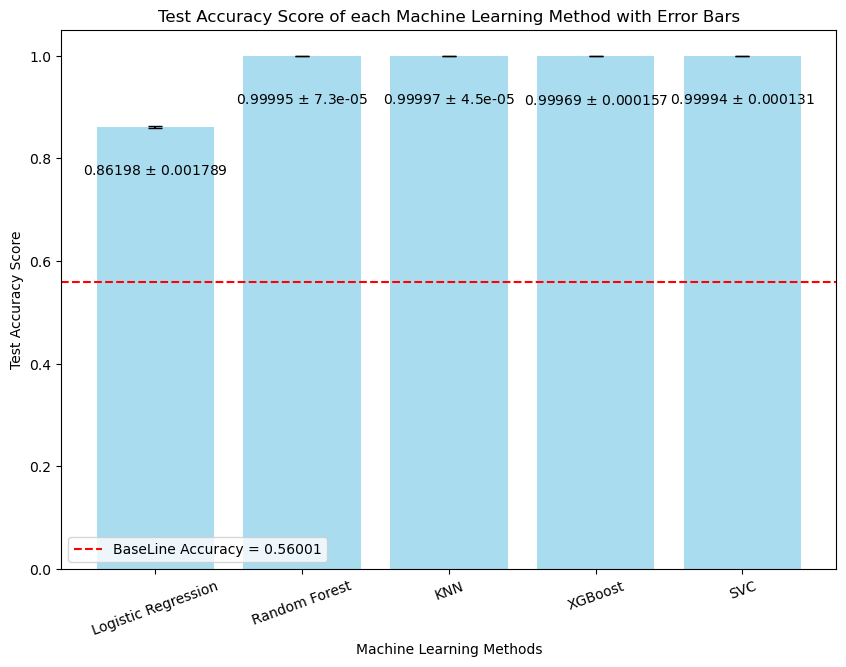
\includegraphics[width=\linewidth]{errorbar1_label.png}
        \caption{Test Accuracy Score of each Machine Learning Method with Error Bars}
        \label{fig:subfig1}
    \end{subfigure}
    \hfill
    \begin{subfigure}{0.46\textwidth}
        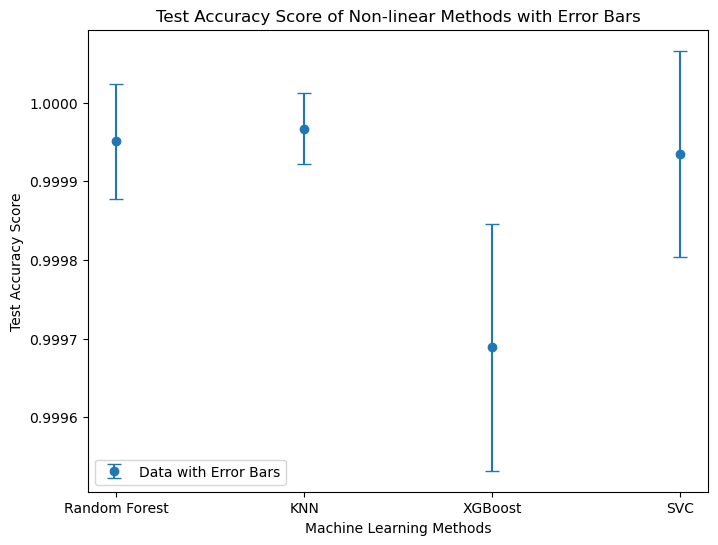
\includegraphics[width=\linewidth]{errorbar2.png}
        \caption{Test Accuracy Score of Non-linear Methods with Error Bars}
        \label{fig:subfig2}
    \end{subfigure}
    \caption{Visualization of Models' Performance with Error Bar.}
    \label{fig:both}
\end{figure}

\begin{table}[h]
\centering
\begin{tabular}{|l|l|l|l|} \hline
\textbf{ML Model} & \textbf{Mean Test Score} & \textbf{Standard Deviation} & \textbf{\# of std above Baseline}\\\hline
Logistic Regression & 0.861978 & 0.001789 & 168.789771\\ \hline
Random Forest & 0.999951 & 0.000073 & 6026.546579 \\ \hline
\textbf{KNN} & \textbf{0.999967} & \textbf{0.000045} & \textbf{9776.753340} \\ \hline
XGBoost & 0.999689 & 0.000157 & 2800.483441 \\ \hline
SVC & 0.999935 & 0.000131 & 3358.182445 \\ \hline
\end{tabular}
\caption{\label{tab:widgets} The performance of the ML models and the corresponding mean test scores, standard deviations, and number of standard deviations above the baseline.}
\end{table}

\newpage
Next, I employ the best model, KNN, to compute the confusion matrix, visualizing the model's performance for each class (see Figure 8). In this confusion matrix, the KNN model with n\_neighbors=3 achieves a perfect accuracy score of 1.0, signifying that all mushrooms in the test set are correctly classified based on their edibility.

\begin{figure}[h]
\centering
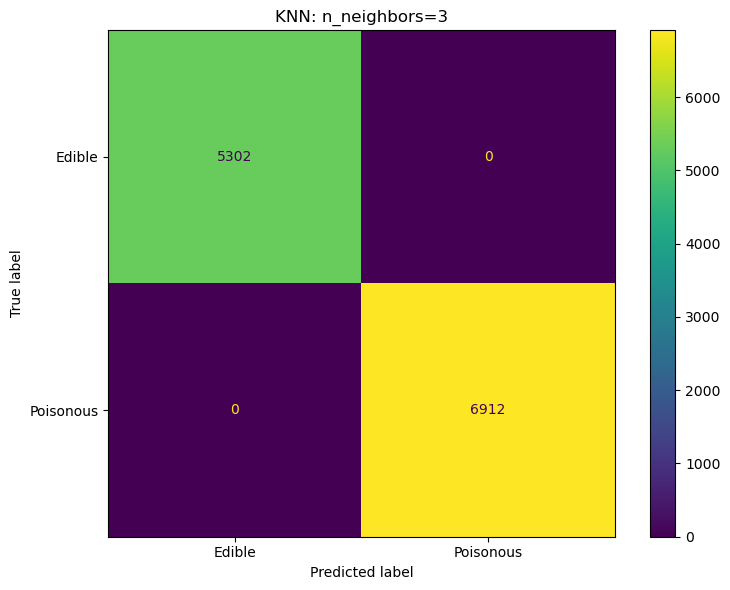
\includegraphics[width=0.75\textwidth]{confusion_matrix_knn_rs=0.png}
\caption{\label{fig:confusion matrix} Confusion Matrix of the best KNN model.}
\end{figure}

\subsection{Feature Importance}
\hspace{0.5cm} To make the model more interpretable, the global and local feature importance can help further understand how each feature contributes to the final prediction.

\subsubsection{Permutation Importance}
\hspace{0.5cm} According to the Permutation Importance figure (see Figure 9),the stem\_height exhibits the largest decrease in performance when its values are permuted, indicating its crucial role in the model's predictive accuracy. Similarly, stem\_width and cap\_diameter features in the dataset also lead to a significant decrease in the model's performance when permuted. In addition, gill\_color and stem\_color also indicate a relatively important role in the prediction.

\begin{figure}[h]
\centering
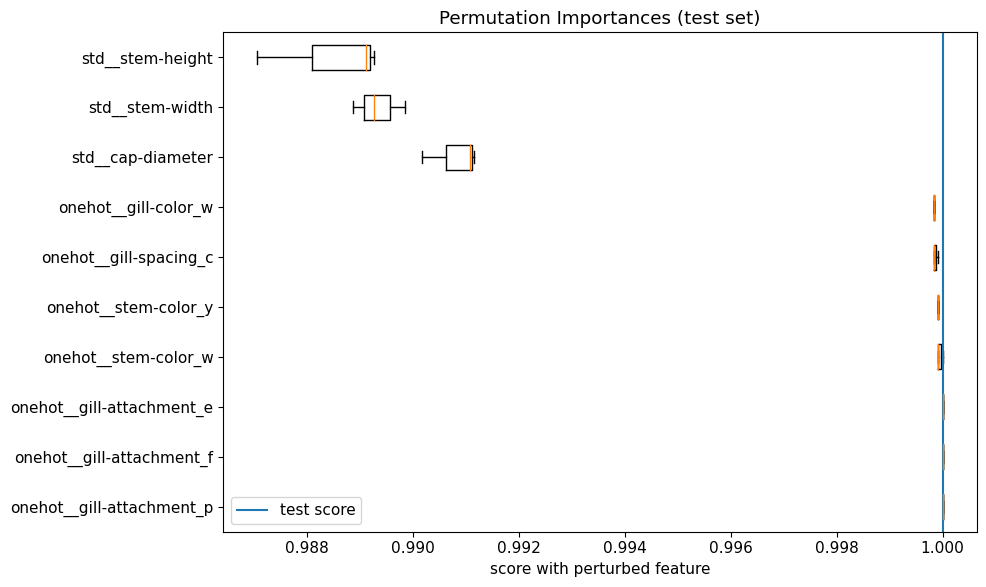
\includegraphics[width=0.85\textwidth]{permutation_knn.png}
\caption{\label{fig:frog} Top 10 Permutation Importance Features.}
\end{figure}

\subsubsection{SHAP values}
\hspace{0.5cm} In this SHAP figure (see Figure 10), the three continuous features - stem\_width, stem\_heigh and cap\_diameter - still play critical roles in the model prediction. Different from the Permutation Importance figure, SHAP metric also considers gill\_attachment and gill\_spacing as one the of critical features.

\begin{figure}[h]
\centering
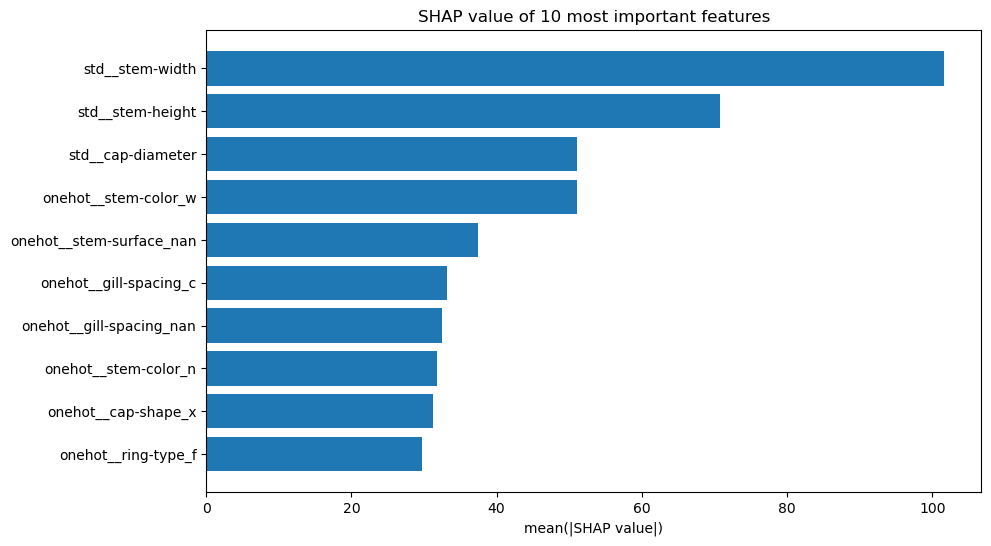
\includegraphics[width=0.85\textwidth]{shap_knn.png}
\caption{\label{fig:frog} Top 10 most important features for mean SHAP values.}
\end{figure}

\subsubsection{Random Forest Feature Importance Based on Mean Decrease in Impurity}
\hspace{0.5cm} The Random Forest Feature Importance is computed as the mean and standard deviation of accumulation of the impurity decrease within each tree. In this Random Forest Feature Importance figure (see Figure 11), similarly, the three continuous features rank the top 3 and following with stem\_color, gill\_spacing and stem\_surface. 

\begin{figure}[h]
\centering
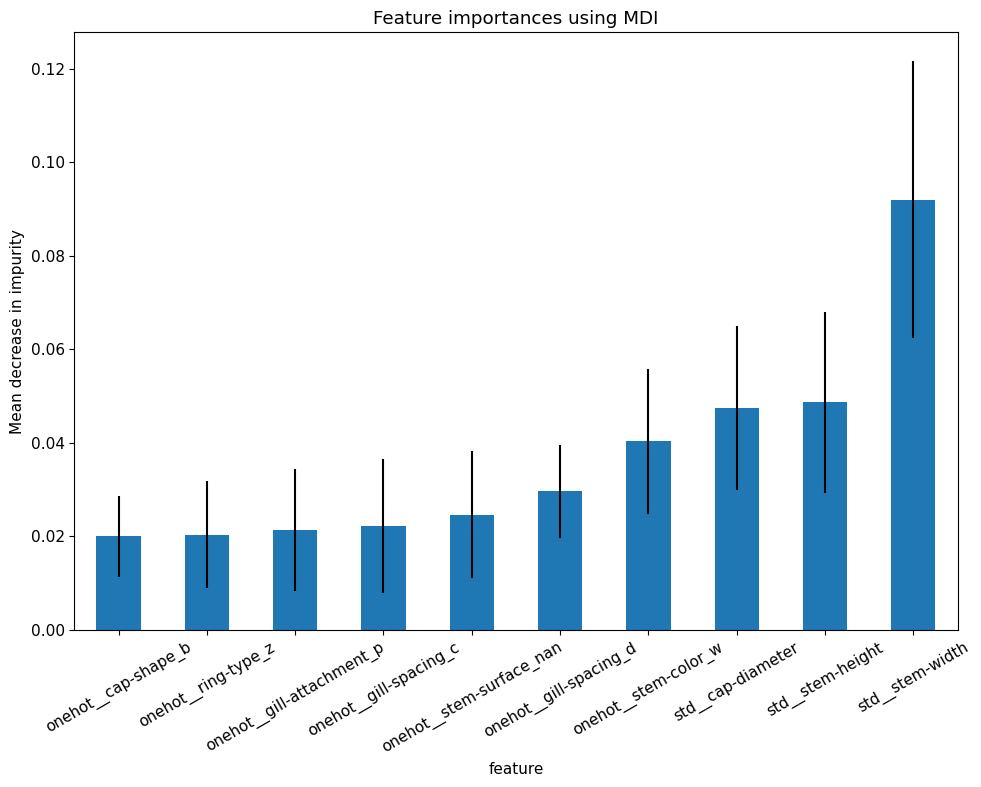
\includegraphics[width=0.8\textwidth]{rf_feature_importance.png}
\caption{\label{fig:frog} Top 10 most important features using MDI in Random Forest.}
\end{figure}

\subsubsection{Force Plot}
\hspace{0.5cm} Using the Force Plots below can help understand how each feature contribute to the final decision of each observation. For the first instance (see Figure 12), the stem\_width, cap\_shape and stem\_surfance indicate the positive contribution to the prediction of the model, strongly suggesting the poisonous nature of this mushroom. Conversely, for the second instance (see Figure 13), the stem\_width, gill\_spacing and gill\_color push the overall decision to the opposite side, indicating that these three features strongly suggest the edibility of this mushroom.

\begin{figure}[h]
\centering
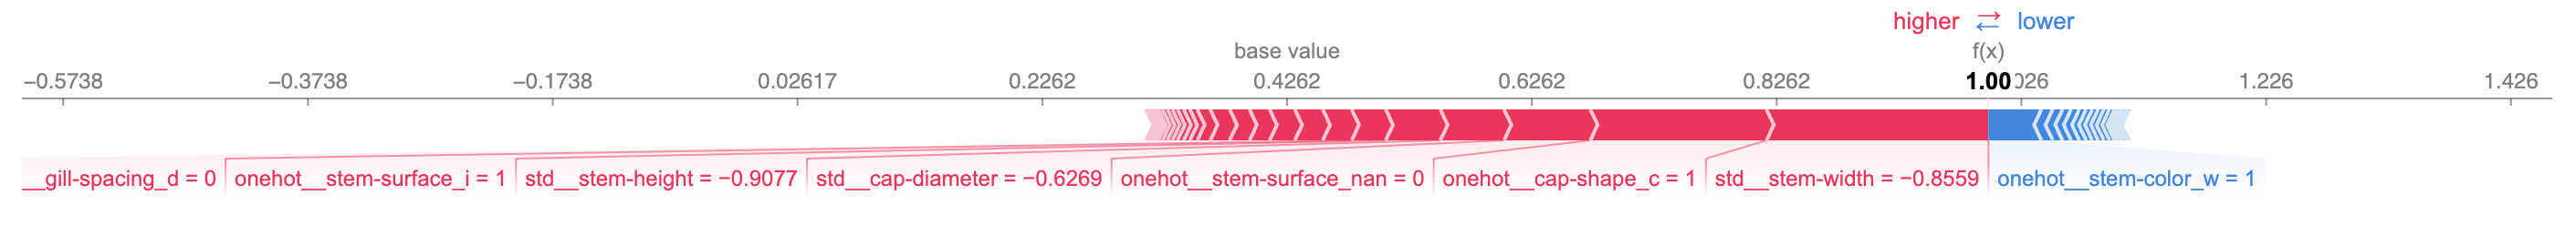
\includegraphics[width=1\textwidth]{local_shp_knn_index=99.png}
\caption{\label{fig:frog} Feature Importance for mushroom with index=99.}
\end{figure}

\begin{figure}[h]
\centering
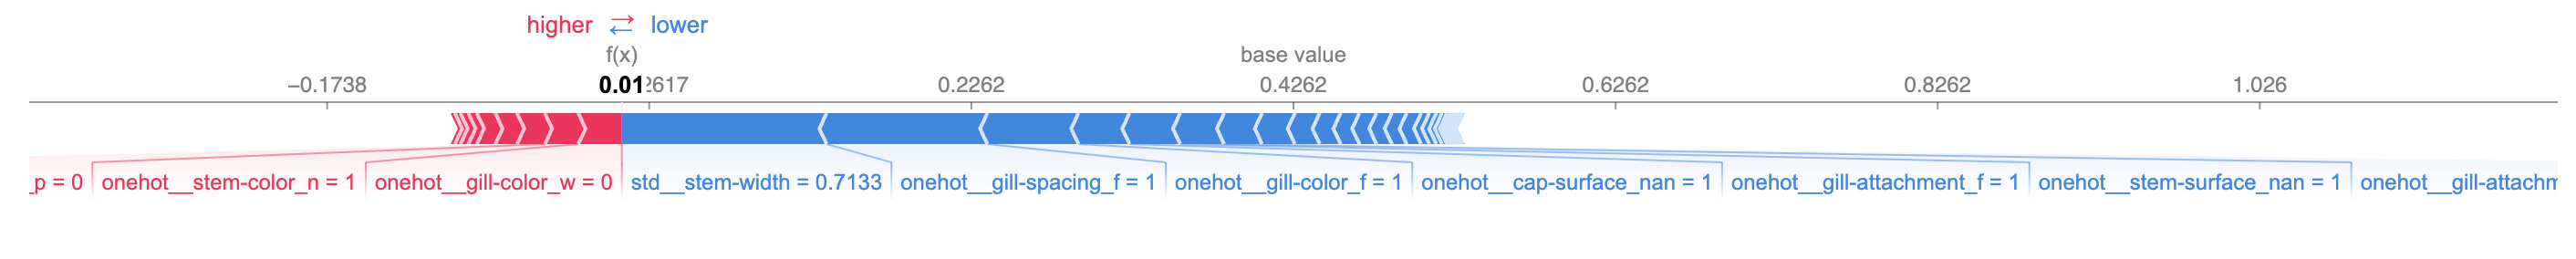
\includegraphics[width=1\textwidth]{local_shap_knn_index=0.png}
\caption{\label{fig:frog} Feature Importance for mushroom with index=0.}
\end{figure}

\subsection{Interesting Finding}
\hspace{0.5cm} After interpreting the feature importance, there is an aspect that aligns with EDA. In the specifically categorized histogram plotting the distribution of stem width based on edibility (see Figure 4), I hypothesize that a mushroom with wider stem width seems to be less pernicious than those with thinner stem width. When examining both force plots for local feature importance (see Figure 12 and Figure 13), the value of stem width for a poisonous mushroom (index=99) is less than 0, indicating a thin stem width. On the other hand, the value of stem width for an edible mushroom (index=0) is greater than 0.5, implying a relatively wider stem width.When interpreting individual predictions, the results from the force plots strongly correlate with the initial hypothesis presented in Figure 4.

\section{Outlook}
\hspace{0.5cm} From the models I currently have, which exhibit strong predictive power, I recognize an opportunity to further enhance interpretability by undertaking feature selection from the pool of 124 features post-preprocessing. While more feature set may contribute to the model's accuracy, it can simultaneously introduce complexity and hinder interpretability. By narrowing down to a more concise set of features, I aim to simplify the model and make its decision-making process more transparent and comprehensible. This streamlined approach not only aids in understanding the critical factors influencing predictions but also makes faster execution reducing the burden on computational power.


\begin{thebibliography}{9}

\bibitem{Li et al.}
Haijiao Li et al.
\textit{Preplanned Studies: Mushroom Poisoning Outbreaks — China, 2022}.
China CDC Weekly, 2023.
DOI: \url{10.46234/ccdcw2023.009}.
Accessed: 7 Dec. 2023.

\bibitem{Zohaib}
Dev Zohaib.
\textit{Mushroom Edibility Classification}.
Kaggle, 2023.
URL: \url{https://www.kaggle.com/datasets/devzohaib/mushroom-edibility-classification}.
Accessed: 7 Dec. 2023.

\bibitem{Payne}
Levi Payne.
\textit{Mushroom Edibility Classification XGBoost}.
Kaggle, 2023.
URL: \url{https://www.kaggle.com/code/levipayne/mushroom-edibility-classification-xgboost}.
Accessed: 7 Dec. 2023.

\bibitem{Agra}
Lucas Agra.
\textit{Mushroom Edibility Classification}.
Kaggle, 2023.
URL: \url{https://www.kaggle.com/code/lucasfca/mushroom-edibility-classification#Conclusion}.
Accessed: 7 Dec. 2023.

\end{thebibliography}


\end{document}